\documentclass[]{article}
\newcommand{\FileDepth}{../../..}
\usepackage[letterpaper, landscape, margin=0.5cm]{geometry}
\usepackage[T1]{fontenc}
\usepackage{textcomp}%Not strictly necessary, but gives \textmu command for "micro."
\usepackage{fancyhdr}
\usepackage{amsmath}
\usepackage{amssymb}
\usepackage{graphicx}
\usepackage{xcolor}
\usepackage{tikz}
\usetikzlibrary{calc}
\usepackage{censor}
\usepackage{hyperref}
\usepackage{multicol}
%opening
\newcommand{\SecType}{L}
\newcommand{\Week}{2}
\title{PH 211 Lecture \Week}
\author{Benjamin Bauml}
\date{Summer 2024}

\newcommand{\Purpose}{4}
\newcommand{\DefOnly}{0}

% Version 2024-06-14
% Changes
% 2024-02-21 Added xstring package to enable smooth implementation of new \ModePage command.
% 2024-04-27 Set up to split activities and formatting aspects into separate files. Removed dependence on xcomment. Added an automatic counter to number the activities in a problem set.
% 2024-05-19 Revised old format for \TeachingTips command, which did not support \DefOnly.
% 2024-06-14 Added Repurpose environment to allow mixing of different purpose levels in the same document.
\usepackage{tcolorbox}
\usepackage{xstring}
% You will want the following four lines in your document (the last two uncommented):
% For Assignment, leave Purpose as 1. For Worksheet, set to 2. For Student Solution, set to 3. For Teacher Solution, set to 4.
% If you want keep the pieces from being called manually, set DefOnly to 0.
%\newcommand{\Purpose}{4}
%\newcommand{\DefOnly}{1}
\newcommand{\Exclusion}{0}
\newcommand{\PageTurn}{0}
\newcommand{\GrayProb}{0}
\newcommand{\Tipsy}{0}

% Assignment
\if\Purpose1
\renewcommand{\Exclusion}{1}
\fi
% Worksheet
\if\Purpose2
\renewcommand{\Exclusion}{1}
\renewcommand{\PageTurn}{1}
\fi
% Student Solution
\if\Purpose3
\renewcommand{\PageTurn}{1}
\renewcommand{\GrayProb}{1}
\fi
% Teaching Copy
\if\Purpose4
\renewcommand{\PageTurn}{1}
\renewcommand{\GrayProb}{1}
\renewcommand{\Tipsy}{1}
\fi

\newenvironment{Repurpose}[1]{
\renewcommand{\Purpose}{#1}
\renewcommand{\Exclusion}{0}
\renewcommand{\PageTurn}{0}
\renewcommand{\GrayProb}{0}
\renewcommand{\Tipsy}{0}
% Assignment
\if\Purpose1
\renewcommand{\Exclusion}{1}
\fi
% Worksheet
\if\Purpose2
\renewcommand{\Exclusion}{1}
\renewcommand{\PageTurn}{1}
\fi
% Student Solution
\if\Purpose3
\renewcommand{\PageTurn}{1}
\renewcommand{\GrayProb}{1}
\fi
% Teaching Copy
\if\Purpose4
\renewcommand{\PageTurn}{1}
\renewcommand{\GrayProb}{1}
\renewcommand{\Tipsy}{1}
\fi
}{}

\def \NewQ {0}
\def \PForce {0}
\newcommand{\MaybePage}[1]{
	\def \PForce {#1}
	\if\PForce1
	\newpage
	\else
	\if\NewQ0
	\gdef \NewQ {\PageTurn}
	\else
	\newpage
	\fi
	\fi
}

\newcommand{\ModePage}[1]{
	\IfSubStr{#1}{\Purpose}{\newpage}{}
}

\newcounter{ActNumber}
\setcounter{ActNumber}{0}

\newcommand{\Problem}[4][0]{%The first argument is optional, and if it is set to 1, the \newpage will be forced. The second argument is the name of the activity, the third is the command the activity is stored as, and the fourth is the actual problem statement.
\newcommand{#3}{
\MaybePage{#1}
\addtocounter{ActNumber}{1}
\section*{\SecType\Week-\theActNumber: #2}
\if\GrayProb1
\begin{tcolorbox}[colback=lightgray,colframe=lightgray,sharp corners,boxsep=1pt,left=0pt,right=0pt,top=0pt,bottom=0pt,after skip=2pt]
\else
\begin{tcolorbox}[colback=white,colframe=white,sharp corners,boxsep=1pt,left=0pt,right=0pt,top=0pt,bottom=0pt,after skip=2pt]
\fi
#4
\end{tcolorbox}\noindent
}
\if\DefOnly0
\else
#3
\fi
}
	
\newcommand{\ProblemSub}[3][0]{%The first argument is optional, and if a string of numbers is entered into it, it will force a \newpage in any \Purpose that shows up in the string. For example, "13" would lead to the newpage being forced in modes 1 and 3. The second is the command the activity is stored as, and the third is the actual problem statement.
\newcommand{#2}{
\ModePage{#1}
\if\GrayProb1
\begin{tcolorbox}[colback=lightgray,colframe=lightgray,sharp corners,boxsep=1pt,left=0pt,right=0pt,top=0pt,bottom=0pt,after skip=2pt]
\else
\begin{tcolorbox}[colback=white,colframe=white,sharp corners,boxsep=1pt,left=0pt,right=0pt,top=0pt,bottom=0pt,after skip=2pt]
\fi
#3
\end{tcolorbox}\noindent
}
\if\DefOnly0
\else
#2
\fi
}
		
\newcommand{\Solution}[2]{%The first argument is the command the solution is stored as, and the second is the actual solution.
\newcommand{#1}{
\if\Exclusion0
#2
\fi
}
\if\DefOnly0
\else
#1
\fi
}
		
\newcommand{\ProblemFig}[2]{%The first argument is the command the figure is stored as, and the second is the actual figure.
\newcommand{#1}{
\begin{figure}[h]
#2
\end{figure}
}
\if\DefOnly0
\else
#1
\fi
}

\newcommand{\TeachingTips}[2]{%The first argument is the command the tip is stored as, and the second is the actual tip.
\newcommand{#1}{
\if\Tipsy1
\begin{tcolorbox}[colback=lightgray,colframe=black]
#2
\end{tcolorbox}
\fi
}
\if\DefOnly0
\else
#1
\fi
}
\usepackage[absolute]{textpos}
% This package relies on Assignment Format 2024-06-14 or later to work. It is recommended that the Purpose and DefOnly commands be given as such:
%\newcommand{\Purpose}{4}
%\newcommand{\DefOnly}{0}
% Activities need to be entered outside of the TeacherMargin and PresentSpace environments, otherwise they will be defined only locally. They can even go in the preamble.
\newenvironment{TeacherMargin}{\begin{textblock*}{10.8cm}(0.5cm,0.5cm)
\small}{\end{textblock*}
\hspace{0.1cm}}
\newenvironment{PresentSpace}{\begin{textblock*}{0.3cm}(26.85cm,9.35cm)
--
\end{textblock*}
\begin{textblock*}{0.3cm}(26.85cm,18.7cm)
--
\end{textblock*}
\begin{textblock*}{0.3cm}(26.85cm,12.24cm)
	--
\end{textblock*}
\begin{textblock*}{15.6cm}(11.8cm,0.5cm)
\begin{Repurpose}{1}
\Large}{\end{Repurpose}
\end{textblock*}
\hspace{0.1cm}}

%\newcommand{\FBDaxes}[3]{
	\begin{scope}[shift={(#1)},rotate=#2]
		% x-axis
		\draw[thick,->] (-2,0) -- (2,0);
		\node[anchor=west] at (2,0) {$x$};
		% y-axis
		\draw[thick,->] (0,-2) -- (0,2);
		\node[anchor=west] at (0,2) {$y$};
		\coordinate (#3) at (0,0);
	\end{scope}
}
\newcommand{\FBDvectorMA}[4]{
	\begin{scope}[shift={(#1)}]
		\coordinate (#4tip) at ({#2*cos(#3)},{#2*sin(#3)});
		\draw[ultra thick,blue,->] (#1) -- (#4tip);
	\end{scope}
}
\newcommand{\FBDvectorXY}[3]{
	\begin{scope}[shift={(#1)}]
		\coordinate (#3tip) at (#2);
		\draw[ultra thick,blue,->] (0,0) -- (#3tip);
	\end{scope}
}
\newcommand{\FBDdot}[1]{
	\filldraw[black] (#1) circle (3pt);
}
%\newcommand{\MVec}[3][0]{%Creates a momentum vector of length #3 centered at #2 and rotated #1 degrees counterclockwise.
	\begin{scope}[rotate=#1,shift={(#2)}]
		\draw[->,thick] ({-#3/2},0) -- ({#3/2},0);
	\end{scope}
}
\newcommand{\MDot}[1]{%Creates a dot at #1 to represent a zero vector.
	\filldraw (#1) circle (1pt);
}
\newcommand{\MVDRows}[2][4.5]{%Creates the rows (initial, delta, final) of a momentum vector diagram. The optional argument determines the width of the table, and defaults to a good length for three columns (two objects and the total system). The non-optional argument gives a coordinate name (not displayed) to the diagram.
	\begin{scope}
		%\draw[thick] (0,5.5) -- (0,0);
		\draw[thick] (-1,4.5) -- (#1,4.5);
		\node at (-0.5,3.75) {$\vec{p}_{i}$};
		\draw[thick] (-1,3) -- (#1,3);
		\node at (-0.5,2.25) {$\Delta\vec{p}$};
		\draw[thick] (-1,1.5) -- (#1,1.5);
		\node at (-0.5,0.75) {$\vec{p}_{f}$};
		\coordinate (#2) at (0,5);
	\end{scope}
}
\newcommand{\MVDCol}[4][0.75]{%Creates a column for an object in a momentum vector diagram. The first (non-optional) argument is the coordinate name (not displayed) of the column, while the second is the displayed column header. The first argument also names the three entries down the column. The third argument anchors the column, so it should either be the coordinate name of the MVD (for the first column) or the coordinate name of the previous column. The optional argument indicates how far the center of the column should be from the previous column's edge, and defaults to 0.75
	\begin{scope}[shift={(#4)}]
		\node at (#1,0) {#3};
		%\draw[thick] ({#1*2},0.5) -- ({#1*2},-5);
		\draw[thick] (0,0.5) -- (0,-5);
		\coordinate (#2init) at (#1,-1.25);
		\coordinate (#2delt) at (#1,-2.75);
		\coordinate (#2fin) at (#1,-4.25);
		\coordinate (#2) at ({#1*2},0);
	\end{scope}
}

%\input{\FileDepth/Activities/Activity_One/Activity_One.tex}
%\input{\FileDepth/Activities/Activity_Two/Activity_Two.tex}

\begin{document}
\begin{TeacherMargin}

\end{TeacherMargin}
\begin{PresentSpace}
\begin{center}
	\huge Lecture 2: Motion
\end{center}
\vspace{1cm}
THREE IMPORTANT STEPS:
\begin{enumerate}
	\item Grab a small whiteboard for yourself! (These are by the doors.)
	\item Sit at tables 2, 3, 6, and 7 (the four closest to the center).
	\item Grab three large whiteboards for your table!
\end{enumerate}
\textbf{I will be randomizing your groups today.}
\end{PresentSpace}
%\newpage
\begin{comment}
\noindent\textbf{From the Syllabus}

Projects are assignments where you will demonstrate and synthesize what you have learned over many weeks. Projects may take many different potential forms, including written, visual, or video. Almost every week (except for weeks with ungrading), there will be some milestone to complete in this project, such as setting group expectations (if you work in a group), proposing a project, submitting a rough draft, peer reviewing other classmates’ projects, and submitting a final draft. All project milestones are due on Fridays.

The standard format for projects that you can expect if you continue on to 212 is a group assignment (usually 3 students), consisting of a 10-15 minute video solution to a physics problem, with a full calculation, sensemaking, and reflection. You may choose to get used to this format in preparation for continuing on in the sequence, or you can take this opportunity to be more creative in how you approach the project. I vehemently encourage you to find some idea for a project that excites you, be it creating an educational video or report, performing research, melding physics with something artistic, or even something I haven’t considered as a possible physics project yet.
\end{comment}
\begin{comment}
\textbf{Project Information}
\begin{itemize}
	\item Demonstrate and synthesize what you have learned over many weeks.
	\item Many possible forms, such as written, visual, or video.
	\item Milestones due Fridays at 8pm (almost) every week:
	\begin{itemize}
		\item Setting group expectations (Week 2)
		\begin{itemize}
			\item Once you have your group, you will work with them in lecture and studio.
		\end{itemize}
		\item Project proposal (Week 3)
		\item Rough draft (Week 5)
		\item Peer review (Week 6)
		\item Final draft (Week 7)
	\end{itemize}
\end{itemize}
\textbf{What to Expect in PH 212}
\begin{itemize}
	\item 10-15 minute video presentation by group (usually 3 students)
	\item Solution to a physics problem, or presentation on self-taught topic (such as buoyant force or drag force)
	\item Calculation, sensemaking, and reflection
\end{itemize}
\textbf{Your Options}
\begin{itemize}
	\item 212 format (get used to it for 212)
	\item Some other idea that excites you!
	\begin{itemize}
		\item Educational video or report
		\item Research
		\item Melding physics with something artistic
		\item Surprise me!
	\end{itemize}
	\item If it doesn't involve enough calculation, sensemaking, and reflection, I may request modifications.
\end{itemize}
\end{comment}
\newpage
\begin{TeacherMargin}

\end{TeacherMargin}
\begin{PresentSpace}
\textbf{A Model for Motion}
\begin{multicols}{2}
	Quantities
	\begin{itemize}
		\item Position: $\vec{r}$
		\item Velocity: $\vec{v}=\frac{d\vec{r}}{dt}$
		\item Acceleration: $\vec{a}=\frac{d\vec{v}}{dt}$
	\end{itemize}
	\vspace{1cm}
	Assumptions
	\begin{itemize}
		\item Use the Particle Model
	\end{itemize}
\end{multicols}
Motion Diagram
\begin{figure}[h]
	\centering
	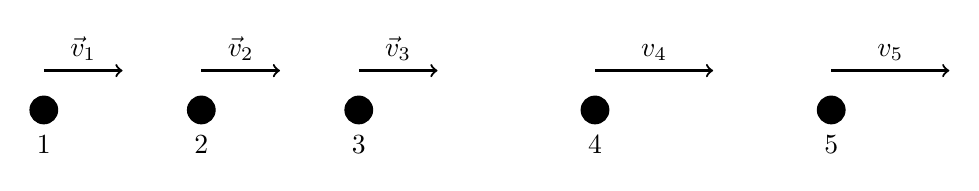
\begin{tikzpicture}
		\foreach \x in {1,2,3}
			\filldraw (2*\x,0) circle (5pt);
		\foreach \x in {1,2,3}
			\node[anchor=north] at (2*\x,-0.2) {\x};
		\foreach \x in {1,2,3}
			\draw[thick,->] (2*\x,0.5) -- (2*\x+1,0.5);
		\foreach \x in {1,2,3}
			\node[anchor=south] at (2*\x+0.5,0.5) {$\vec{v}_{\x}$};
		\begin{scope}[shift={(-3,0)}]
			\foreach \x in {4,5}
				\filldraw (3*\x,0) circle (5pt);
			\foreach \x in {4,5}
				\node[anchor=north] at (3*\x,-0.2) {\x};
			\foreach \x in {4,5}
				\draw[thick,->] (3*\x,0.5) -- (3*\x+1.5,0.5);
			\foreach \x in {4,5}
				\node[anchor=south] at (3*\x+0.75,0.5) {$v_{\x}$};
		\end{scope}
	\end{tikzpicture}
\end{figure}
\end{PresentSpace}
\newpage
\begin{TeacherMargin}
\noindent\textbf{Explanations}

\noindent\textbf{L2-1: Comparing Motion Diagrams}

\noindent\textbf{Principles}
\begin{itemize}
	\item $\vec{v}_{avg} = \frac{\Delta\vec{r}}{\Delta t}$
	\item For a motion diagram, the time intervals are the same.
\end{itemize}
\noindent\textbf{Reasoning}

\noindent\textit{Method 1:}

Let us look at the beginning and end of the motion. Each object starts and ends at the same spot:
\[
\Delta\vec{r}_{1} = \Delta\vec{r}_{2} = \Delta\vec{r}.
\]
Object 2 takes more time to get to the final position:
\[
\Delta t_{2} > \Delta t_{1}.
\]
Now we have
\[
\vec{v}_{avg,1} = \frac{\Delta\vec{r}_{1}}{\Delta t_{1}}, \qquad \vec{v}_{avg,2} = \frac{\Delta\vec{r}_{2}}{\Delta t_{2}}.
\]
Since $\Delta\vec{r}$ is the same for both, a larger number in the denominator gives a smaller overall number. Therefore
\[
\left|\vec{v}_{avg,1}\right| > \left|\vec{v}_{avg,2}\right|.
\]

\noindent\textit{Method 2:}

Since the velocity appears to be constant (that is, $\Delta\vec{r}$ between two adjacent spots is the same), we can also look at individual positions.

For object 1, $\Delta\vec{r}$ between times 1 and 2 is greater than for object 2:
\[
\Delta\vec{r}_{1} > \Delta\vec{r}_{2}.
\]
The time between these two points is the same for both objects:
\[
\Delta t_{1} = \Delta t_{2} = \Delta _{t}.
\]
Now we have
\[
\vec{v}_{avg,1} = \frac{\Delta\vec{r}_{1}}{\Delta t}, \qquad \vec{v}_{avg,2} = \frac{\Delta\vec{r}_{2}}{\Delta t}.
\]
The denominators are the same, so having a larger number in the numerator gives a larger overall number. Therefore
\[
\left|\vec{v}_{avg,1}\right| > \left|\vec{v}_{avg,2}\right|.
\]

\noindent\textbf{Conclusion}

The average speed of object 1 is \underline{greater than} the average speed of object 2:
\[
\left|\vec{v}_{avg,1}\right| > \left|\vec{v}_{avg,2}\right|.
\]
\end{TeacherMargin}
\begin{PresentSpace}
\vspace{-0.5cm}
\section*{L2-1: Comparing Motion Diagrams}
\vspace{-0.2cm}
The diagrams below show the motion of two different objects. Is the average velocity of the upper object greater than, less than, or equal to the average velocity of the lower object? Explain your reasoning.
\vspace{0.3cm}
\begin{figure}[h]
	\centering
	\begin{tikzpicture}
		\node at (0.75,0) {Object 1};
		\foreach \x in {1,2,3,4,5}
			\filldraw (3*\x,0) circle (5pt);
		\foreach \x in {1,2,3,4,5}
			\node[anchor=north] at (3*\x,-0.2) {\x};
		\begin{scope}
			\node at (0.75,-1.5) {Object 2};
			\foreach \x in {1,2,3,4,5,6}
				\filldraw (2.4*\x+0.6,-1.5) circle (5pt);
			\foreach \x in {1,2,3,4,5,6}
				\node[anchor=north] at (2.4*\x+0.6,-1.7) {\x};
		\end{scope}
		\node at (7.5,-4) {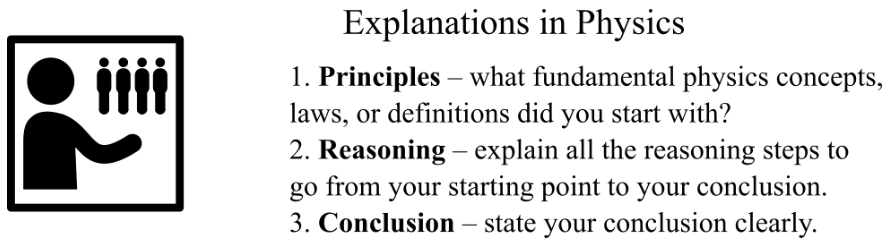
\includegraphics[scale=0.4]{ExplanationsInPhysics.png}};
	\end{tikzpicture}
\end{figure}
\end{PresentSpace}
\newpage
\begin{TeacherMargin}
\noindent\textbf{L2-2 Thrown Ball}

The ball goes up, slows down, comes to a brief stop, turns around, and falls back down, increasing in speed.

\noindent\textbf{Analyze and Represent}

\noindent\textbf{1a: Understand the Problem}
\begin{itemize}
	\item $\vec{r}$: position of the ball (subscripts will denote which point in time the position corresponds to)
	\item $\vec{v}$: velocity of the ball (subscripts will denote which point in time the position corresponds to)
	\item $\vec{r}_{1}$: initial position
	\item $\vec{v}_{1}$: initial velocity
	\item $\vec{r}_{7}$: final position
	\item $\vec{v}_{7}$: final velocity
	\item $t$: time
\end{itemize}
\noindent\textbf{1b: Identify Assumptions}
\begin{itemize}
	\item The ball is thrown in a straight line.
	\begin{itemize}
		\item This simplification allows us to consider motion in only one dimension.
	\end{itemize}
	\item The ball is released and caught at the same spot.
	\begin{itemize}
		\item An actual toss and catch isn't going to be perfect, but small, random differences in starting and ending height are a minor detail that we don't need to bother with when looking at this general sort of motion.
	\end{itemize}
	\item Particle model.
	\begin{itemize}
		\item This assumption allows us to ignore any ambiguity in the object's position (we don't have to decide to measure from the center, top, or bottom), and to ignore any rotational motion the object may have about its own axis.
	\end{itemize}
\end{itemize}
\noindent\textbf{1c: Represent Physically}

A motion diagram can help us visualize the motion of the ball. The velocity vectors (based on forward approximation) give us a sense of how fast the ball is moving at each time.

\begin{figure}[h]
	\centering
	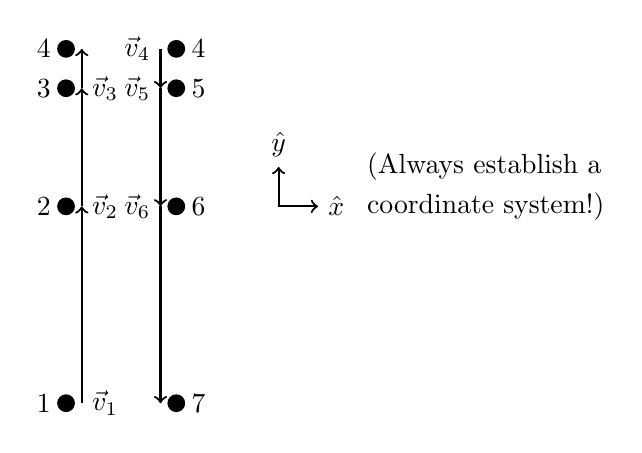
\begin{tikzpicture}
		\begin{scope}[shift={(-3.7,0)}]
			\foreach \t in {1,2,3,4}
				\filldraw (0,{-0.5*(\t-4)*(\t-4)}) circle (3pt) node[anchor=east,shift={(-2pt,0)}] {$\t$};
			\foreach \t in {1,2,3}
				\draw[thick,->] (0.2,{-0.5*(\t-4)*(\t-4)}) node[anchor=west,shift={(0,0)}] {$\vec{v}_{\t}$} -- (0.2,{-0.5*(\t-3)*(\t-3)});
		\end{scope}
		\begin{scope}[shift={(-2.3,0)}]
			\foreach \t in {4,5,6,7}
				\filldraw (0,{-0.5*(\t-4)*(\t-4)}) circle (3pt) node[anchor=west,shift={(2pt,0)}] {$\t$};
			\foreach \t in {4,5,6}
				\draw[thick,->] (-0.2,{-0.5*(\t-4)*(\t-4)}) node[anchor=east,shift={(0,0)}] {$\vec{v}_{\t}$} -- (-0.2,{-0.5*(\t-3)*(\t-3)});
		\end{scope}
		\begin{comment}[shift={(-0.8,0)}]
			\foreach \t in {1,2,3,4}
				\filldraw (0,{-0.5*(\t-4)*(\t-4)}) circle (3pt) node[anchor=east,shift={(-2pt,0)}] {$\t$};
			\foreach \t in {1,2,3}
				\draw[thick,->] (0.1*\t+0.1,{-0.5*(\t-4)*(\t-4)}) node[anchor=west,shift={(0,0)}] {$\vec{v}_{\t}$} -- (0.1*\t+0.1,{-0.25*(\t-3)*(\t-3)+0.25*(\t-5)*(\t-5)-0.5*(\t-4)*(\t-4)});
		\end{comment}
		%\node at (0.2,0.3) {$\vec{v}_{4}=\vec{0}$};
		\begin{comment}[shift={(0.8,0)}]
			\foreach \t in {4,5,6,7}
				\filldraw (0,{-0.5*(\t-4)*(\t-4)}) circle (3pt) node[anchor=west,shift={(2pt,0)}] {$\t$};
			\foreach \t in {5,6,7}
				\draw[thick,->] (-0.2,{-0.5*(\t-4)*(\t-4)}) node[anchor=east,shift={(0,0)}] {$\vec{v}_{\t}$} -- (-0.2,{-0.25*(\t-3)*(\t-3)+0.25*(\t-5)*(\t-5)-0.5*(\t-4)*(\t-4)});
		\end{comment}
		\begin{comment}[shift={(2.3,0)}]
			\foreach \t in {1,2,3,4}
				\filldraw (0,{-0.5*(\t-4)*(\t-4)}) circle (3pt) node[anchor=east,shift={(-2pt,0)}] {$\t$};
			\foreach \t in {2,3}
				\draw[thick,->] (0.1*\t,{-0.5*(\t-4)*(\t-4)}) node[anchor=west,shift={(0,0)}] {$\vec{v}_{\t}$} -- (0.1*\t,{-(\t-4)*(\t-4)+0.5*(\t-5)*(\t-5)});
		\end{comment}
		\begin{comment}[shift={(3.7,0)}]
			\foreach \t in {4,5,6,7}
				\filldraw (0,{-0.5*(\t-4)*(\t-4)}) circle (3pt) node[anchor=west,shift={(2pt,0)}] {$\t$};
			\foreach \t in {4,5,6,7}
				\draw[thick,->] (-0.2,{-0.5*(\t-4)*(\t-4)}) node[anchor=east,shift={(0,0)}] {$\vec{v}_{\t}$} -- (-0.2,{-(\t-4)*(\t-4)+0.5*(\t-5)*(\t-5)});
		\end{comment}
		\begin{scope}[shift={(-1,-2)}]
			\draw[thick,<->] (0.5,0) node[anchor=west] {$\hat{x}$} -- (0,0) -- (0,0.5) node[anchor=south] {$\hat{y}$};
		\end{scope}
		\node[anchor=west] at (0,-1.5) {(Always establish a};
		\node[anchor=west] at (0,-2) {coordinate system!)};
	\end{tikzpicture}
\end{figure}
\end{TeacherMargin}
\begin{PresentSpace}
\vspace{-0.5cm}
\section*{L2-2: Thrown Ball}
\vspace{-0.2cm}
A ball is thrown straight into the air.
\begin{itemize}
	\item Describe the motion in words (use complete sentences).
	\item Identify any quantities of interest with a symbol.
	\item Draw a motion diagram for the ball.
	\item Discuss any assumptions or idealizations you want to make.
\end{itemize}
\vspace{12cm}
\begin{figure}[h]
	\centering
	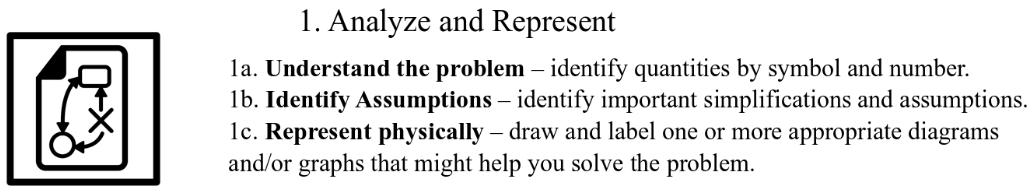
\includegraphics[scale=0.4]{AnalyzeAndRepresent.png}
\end{figure}
\end{PresentSpace}
\newpage
\begin{TeacherMargin}
\noindent\textbf{Forward Approximation}

The velocity at time $t_{j}$ is approximated as the average velocity from $t_{j}$ to $t_{j+1}$:
\[
\vec{v}_{j} \approx \frac{\vec{r}_{j+1}-\vec{r}_{j}}{\Delta t}
\]
Note that this means we can't give a velocity to the final dot, as there is no next dot to get a final position from.

\noindent\textbf{Backward Approximation}

The velocity at time $t_{j}$ is approximated as the average velocity from $t_{j-1}$ to $t_{j}$:
\[
\vec{v}_{j} \approx \frac{\vec{r}_{j}-\vec{r}_{j-1}}{\Delta t}
\]
This time, we can't give a velocity to the first dot, as there is no previous dot to get an initial position from.

\noindent\textbf{Balanced Approximation}

The velocity at time $t_{j}$ is approximated as the average velocity from $t_{j-1}$ to $t_{j+1}$:
\[
\vec{v}_{j} \approx \frac{\vec{r}_{j+1}-\vec{r}_{j-1}}{2\Delta t}
\]
Now, we can't give a velocity to either the first or last dot. Note that we are looking two dots apart, so the time interval is doubled.

\noindent\textbf{Instantaneous}

Here, the velocity is actually calculated as the derivative of a known position equation. Note that the velocities from the balanced approximation is extremely close to the instantaneous velocities in this situation.

\noindent\textbf{Motion Graph}

A motion diagram overlays snapshots of the object at different times into a single picture. A motion graph gives time an axis of its own. Each point on the graph has the same $y$ separation as the corresponding points in the motion diagram, but they now also have a separation in $t$ that clarifies at what point they happen in time.

The forward and backward approximations are a bit rough, whereas the balanced approximation is close to the instantaneous velocity. It is still an approximation, though, so it is not perfect.

The approximations of $\vec{v}_{2}$ were brought out from the graph for clarity. The backward approximation is too steep (giving too large of a velocity), and the forward approximation is not steep enough (giving too small of a velocity).

\end{TeacherMargin}
\begin{PresentSpace}
\noindent\textbf{Motion Diagrams}

\begin{figure}[h]
	\centering
	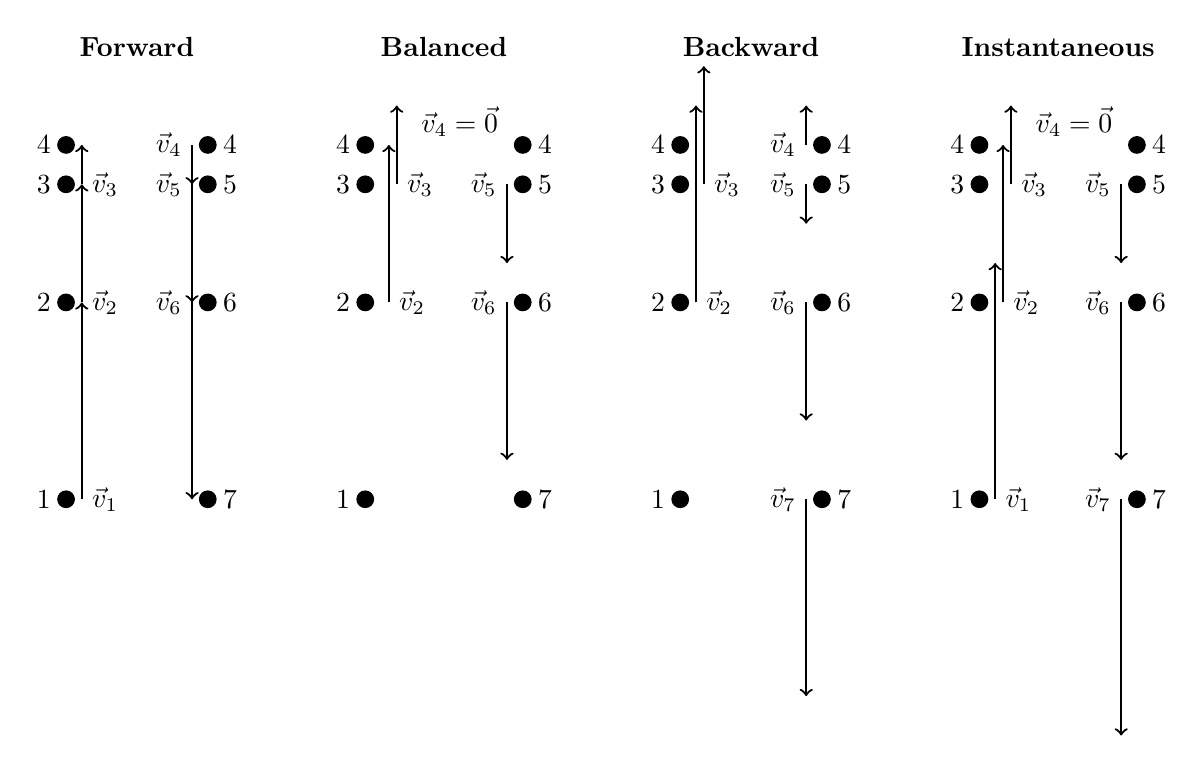
\begin{tikzpicture}
		\node at (-3.9,1.25) {\textbf{Forward}};
		\begin{scope}[shift={(-4.8,0)}]
			\foreach \t in {1,2,3,4}
				\filldraw (0,{-0.5*(\t-4)*(\t-4)}) circle (3pt) node[anchor=east,shift={(-2pt,0)}] {$\t$};
			\foreach \t in {1,2,3}
				\draw[thick,->] (0.2,{-0.5*(\t-4)*(\t-4)}) node[anchor=west,shift={(0,0)}] {$\vec{v}_{\t}$} -- (0.2,{-0.5*(\t-3)*(\t-3)});
		\end{scope}
		\begin{scope}[shift={(-3,0)}]
			\foreach \t in {4,5,6,7}
				\filldraw (0,{-0.5*(\t-4)*(\t-4)}) circle (3pt) node[anchor=west,shift={(2pt,0)}] {$\t$};
			\foreach \t in {4,5,6}
				\draw[thick,->] (-0.2,{-0.5*(\t-4)*(\t-4)}) node[anchor=east,shift={(0,0)}] {$\vec{v}_{\t}$} -- (-0.2,{-0.5*(\t-3)*(\t-3)});
		\end{scope}
		\node at (0,1.25) {\textbf{Balanced}};
		\begin{scope}[shift={(-1,0)}]
			\foreach \t in {1,2,3,4}
				\filldraw (0,{-0.5*(\t-4)*(\t-4)}) circle (3pt) node[anchor=east,shift={(-2pt,0)}] {$\t$};
			\foreach \t in {2,3}
				\draw[thick,->] (0.1*\t+0.1,{-0.5*(\t-4)*(\t-4)}) node[anchor=west,shift={(0,0)}] {$\vec{v}_{\t}$} -- (0.1*\t+0.1,{-0.25*(\t-3)*(\t-3)+0.25*(\t-5)*(\t-5)-0.5*(\t-4)*(\t-4)});
		\end{scope}
		\node at (0.2,0.3) {$\vec{v}_{4}=\vec{0}$};
		\begin{scope}[shift={(1,0)}]
			\foreach \t in {4,5,6,7}
				\filldraw (0,{-0.5*(\t-4)*(\t-4)}) circle (3pt) node[anchor=west,shift={(2pt,0)}] {$\t$};
			\foreach \t in {5,6}
				\draw[thick,->] (-0.2,{-0.5*(\t-4)*(\t-4)}) node[anchor=east,shift={(0,0)}] {$\vec{v}_{\t}$} -- (-0.2,{-0.25*(\t-3)*(\t-3)+0.25*(\t-5)*(\t-5)-0.5*(\t-4)*(\t-4)});
		\end{scope}
		\node at (3.9,1.25) {\textbf{Backward}};
		\begin{scope}[shift={(3,0)}]
			\foreach \t in {1,2,3,4}
				\filldraw (0,{-0.5*(\t-4)*(\t-4)}) circle (3pt) node[anchor=east,shift={(-2pt,0)}] {$\t$};
			\foreach \t in {2,3}
				\draw[thick,->] (0.1*\t,{-0.5*(\t-4)*(\t-4)}) node[anchor=west,shift={(0,0)}] {$\vec{v}_{\t}$} -- (0.1*\t,{-(\t-4)*(\t-4)+0.5*(\t-5)*(\t-5)});
		\end{scope}
		\begin{scope}[shift={(4.8,0)}]
			\foreach \t in {4,5,6,7}
				\filldraw (0,{-0.5*(\t-4)*(\t-4)}) circle (3pt) node[anchor=west,shift={(2pt,0)}] {$\t$};
			\foreach \t in {4,5,6,7}
				\draw[thick,->] (-0.2,{-0.5*(\t-4)*(\t-4)}) node[anchor=east,shift={(0,0)}] {$\vec{v}_{\t}$} -- (-0.2,{-(\t-4)*(\t-4)+0.5*(\t-5)*(\t-5)});
		\end{scope}
		\begin{scope}[shift={(7.8,0)}]
			\node at (0,1.25) {\textbf{Instantaneous}};
			\begin{scope}[shift={(-1,0)}]
				\foreach \t in {1,2,3,4}
					\filldraw (0,{-0.5*(\t-4)*(\t-4)}) circle (3pt) node[anchor=east,shift={(-2pt,0)}] {$\t$};
				\foreach \t in {1,2,3}
					\draw[thick,->] (0.1*\t+0.1,{-0.5*(\t-4)*(\t-4)}) node[anchor=west,shift={(0,0)}] {$\vec{v}_{\t}$} -- (0.1*\t+0.1,{-1*(\t-4)-0.5*(\t-4)*(\t-4)});
			\end{scope}
			\node at (0.2,0.3) {$\vec{v}_{4}=\vec{0}$};
			\begin{scope}[shift={(1,0)}]
				\foreach \t in {4,5,6,7}
					\filldraw (0,{-0.5*(\t-4)*(\t-4)}) circle (3pt) node[anchor=west,shift={(2pt,0)}] {$\t$};
				\foreach \t in {5,6,7}
					\draw[thick,->] (-0.2,{-0.5*(\t-4)*(\t-4)}) node[anchor=east,shift={(0,0)}] {$\vec{v}_{\t}$} -- (-0.2,{-1*(\t-4)-0.5*(\t-4)*(\t-4)});
			\end{scope}
		\end{scope}
	\end{tikzpicture}
\end{figure}

\noindent\textbf{Motion Graph}

\begin{figure}[h]
	\centering
	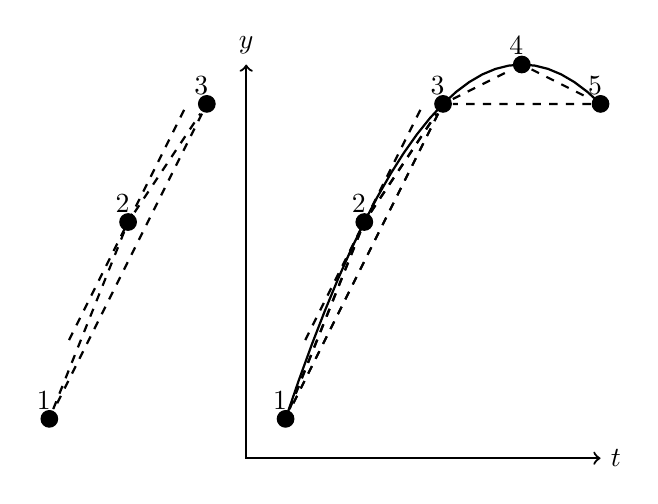
\begin{tikzpicture}
		\draw[thick,<->] (0.5,0) node[anchor=south] {$y$} -- (0.5,-5) -- (5,-5) node[anchor=west] {$t$};
		\draw[thick,domain=1:5,variable=\t] plot ({\t},{-0.5*(\t-4)*(\t-4)});
		\foreach \t in {1,2,3,4,5}
			\filldraw (\t,{-0.5*(\t-4)*(\t-4)}) node  (dot\t) {} circle (3pt) node[anchor=south,shift={(-2pt,0)}] {$\t$};
		\draw[thick,dashed] (dot3) -- (dot4) -- (dot5) -- (dot3);
		\draw[thick,dashed] (dot1) -- (dot2) -- (dot3) -- (dot1);
		\draw[thick,dashed,domain=-0.75:0.75,variable=\t] plot ({\t+2},{2*\t-2});
		\draw[thick,dashed] (dot1) -- (dot2) -- (dot3) -- (dot1);
		\begin{scope}[shift={(-3,0)}]
			\foreach \t in {1,2,3}
				\filldraw (\t,{-0.5*(\t-4)*(\t-4)}) node  (ddot\t) {} circle (3pt) node[anchor=south,shift={(-2pt,0)}] {$\t$};
			\draw[thick,dashed,domain=-0.75:0.75,variable=\t] plot ({\t+2},{2*\t-2});
		\end{scope}
		\draw[thick,dashed] (ddot1) -- (ddot2) -- (ddot3) -- (ddot1);
	\end{tikzpicture}
\end{figure}
\end{PresentSpace}
\newpage
\begin{TeacherMargin}
\noindent\textbf{L2-2 Thrown Ball}

\noindent\textbf{Calculate}

\noindent\textbf{2a: Represent Principles}

Instantaneous velocity at a particular time can be approximated by the average velocity over a span of time containing that particular time:
\[
\vec{v} = \frac{d\vec{r}}{dt} \approx \vec{v}_{avg} = \frac{\Delta\vec{r}}{\Delta t}.
\]

\noindent\textbf{2b: Find unknown(s) Symbolically}

For the entire motion, the average velocity from start to finish is
\[
\vec{v}_{avg} = \frac{\vec{r}_{7}-\vec{r}_{1}}{t_{7}-t_{1}} = 0,
\]
because it starts and ends at the same position ($\vec{r}_{7}=\vec{r}_{1}$)!

For the first half, we can calculate the average velocity from the launch to the peak:
\[
\vec{v}_{avg} = \frac{\vec{r}_{4}-\vec{r}_{1}}{t_{4}-t_{1}}.
\]

For the second half, we can calculate the average velocity from the peak to the catch:
\[
\vec{v}_{avg} = \frac{\vec{r}_{7}-\vec{r}_{4}}{t_{7}-t_{4}}.
\]

At this point, we can already tell that the velocity is not constant. Since $\vec{r}_{1} = \vec{r}_{7}$ and $t_{4}-t_{1} = t_{7}-t_{4}$, we can see that these two velocities are in opposite directions (and even if the vector stays the same magnitude, it is not constant if its direction changes).

\noindent\textbf{2c: Plug in Numbers}

We are not given numbers, so we should estimate some. If I toss an object such that it lands back in my hand after half of a second (so it reaches its maximum height after a quarter of a second), it looks like it gets maybe a foot (so a third of a meter) up in the air.

For the first half of the motion, this gives us
\[
\Delta\vec{r} \approx \left(\frac{1}{3} \text{m}\right) \hat{y}, \qquad \Delta t \approx 0.5 \text{s},
\]
which means $\vec{v}_{avg} \approx \frac{1}{6}\frac{\text{m}}{\text{s}}\hat{y}$. For the second half, we get
\[
\Delta\vec{r} \approx \left(\frac{1}{3} \text{m}\right) \left(-\hat{y}\right), \qquad \Delta t \approx 0.5 \text{s},
\]
which means $\vec{v}_{avg} \approx \frac{1}{6}\frac{\text{m}}{\text{s}}\left(-\hat{y}\right)$.

Note that the direction information is all in the unit vector, as seen by the negative sign. Also, the magnitude carries units, whereas the unit vector does not (which is admittedly a confusing naming issue).
\end{TeacherMargin}
\begin{PresentSpace}
	\vspace{-0.5cm}
	\section*{L2-2: Thrown Ball}
	\vspace{-0.2cm}
	A ball is thrown straight into the air.
	\begin{itemize}
		\item Estimate the average velocity of the ball:
		\begin{itemize}
			\item During the entire motion.
			\item During the first half of the motion.
			\item During the second half of the motion.
		\end{itemize}
		\item Is the velocity constant?
	\end{itemize}
	\vspace{11cm}
	\begin{figure}[h]
		\centering
		
\includegraphics[scale=0.4]{Calculate.png}
	\end{figure}
\end{PresentSpace}
\newpage
\begin{TeacherMargin}
If you want to calculate an estimate of instantaneous acceleration by finding the average acceleration, it works just like calculating average velocity, except it is the difference in velocity that we divide by elapsed time. However, if you are calculating average acceleration from estimates of velocity, your approximation will get worse, since there is error associated wit both calculation results.
\end{TeacherMargin}
\begin{PresentSpace}
\vspace{-0.5cm}
\section*{Acceleration}
\vspace{-0.2cm}
\begin{itemize}
	\item An object that changes in velocity is said to be accelerating.
	\item Acceleration is defined as the change in velocity divided by the change in time.
	\item Average:
	\[
	\vec{a}_{avg} = \frac{\Delta\vec{v}}{\Delta t}
	\]
	\item Instantaneous:
	
	\[
	\vec{a} = \frac{d\vec{v}}{dt}
	\]
\end{itemize}
\end{PresentSpace}
\newpage
\begin{TeacherMargin}

\end{TeacherMargin}
\begin{PresentSpace}
\vspace{-0.5cm}
\section*{Main Ideas}
\vspace{-0.2cm}
\begin{itemize}
	\item The motion of an object can be characterized by quantities like position, velocity, and acceleration.
	\item Velocity is defined as the time rate of change of position.
	\item Acceleration is defined as the time rate of change of velocity.
\end{itemize}
\end{PresentSpace}
\end{document}